\section{Risk Parity Model Based on MVT}
\subsection{Data Selection}
In order to test whether the risk parity model based on MVT can perform well in the actual market, we use the standard deviation(Std), value at risk(VaR), and expected shortfall(ES) as the indicators of risk measurement to construct the risk parity model for CSI 300, CSI ABI and Gold ETF and carry out the dynamic backtesting. In terms of the time duration, we still applied the logarithmic rate of return data from 2015 to 2019. However, due to the need to estimate parameters and calculate risk metrics during the backtesting process, the actual backtesting interval is from April 2015 to December 2019.

\subsection{Model Derivation}
\subsubsection{Consistency in Risk Metrics}
\cite{AP1999Coherentmeasures} gave the concept of consistency of risk measurement: Let $\Omega$ be the set of all possible states of an event, the set $\mathcal{F}$ of all real-valued functions defined on $\Omega$ is called the risk set. The risk measure $\boldsymbol{\mathcal{R}}(.)$ is a mapping from $\mathcal{F}$ to space $\mathbb{R}$. The risk measure is consistent if it satisfies the following properties: 
\begin{itemize}
  \item Monotonicity: $\forall X_1 \geq X_2 \in \mathcal{F}, \mathcal{R}\left(\mathrm{X}_1\right) \geq \mathcal{R}\left(\mathrm{X}_2\right)$ 
  \item Homogeneity: $\forall X \in \mathcal{F}, c \geq 0, \mathcal{R}(\mathrm{cX})=c \mathcal{R}(\mathrm{X})$
  \item Translation Invariance: $\forall X \in \mathcal{F}, c \in \mathbb{R}, \mathcal{R}(\mathrm{X}+\mathrm{c})=\mathcal{R}(\mathrm{X})-c$ 
  \item Subadditivity: $\forall X_1, X_2, \ldots, X_N \in \mathcal{F}, \mathcal{R}\left( \sum_{i=1}^{N} X_i\right) \leq \sum_{i=1}^{N} \mathcal{R}\left(X_i\right)$
\end{itemize}
% \noindent(1) Monotonicity: $\forall X_1 \geq X_2 \in \mathcal{F}, \mathcal{R}\left(\mathrm{X}_1\right) \geq \mathcal{R}\left(\mathrm{X}_2\right)$ \\
% (2) Homogeneity: $\forall X \in \mathcal{F}, c \geq 0, \mathcal{R}(\mathrm{cX})=c \mathcal{R}(\mathrm{X})$ \\
% (3) Translation Invariance: $\forall X \in \mathcal{F}, c \in \mathbb{R}, \mathcal{R}(\mathrm{X}+\mathrm{c})=\mathcal{R}(\mathrm{X})-c$ \\
% (4) Subadditivity: $\forall X_1, X_2, \ldots, X_N \in \mathcal{F}, \mathcal{R}\left( \sum_{i=1}^{N} X_i\right) \leq \sum_{i=1}^{N} \mathcal{R}\left(X_i\right)$

\noindent Whether the risk measurement indicators are consistent plays a vital role in measuring the risk degree of the asset portfolio. Use N assets $X_{1}, X_{2},...X_{N}$ to build an asset portfolio $w=(w_{1},w_{2},...,w_{N} )^T$, where $\sum_{i=1}^N w_i=1$. If the risk measurement index $\mathcal{R}(.)$ has subadditivity and homogeneity, then
$$
    \mathcal{R}\left(\sum_{i=1}^N w_i X_i\right) \leq \sum_{i=1}^N w_i \mathcal{R}\left(X_i\right)
$$
which investors can reduce investment risk by allocating funds in different assets. By definition, the standard deviation is consistent, and the consistency of the expected loss has been proved by \cite{TD2002}.


\subsubsection{Model Extension}
The traditional risk parity model is based on the standard deviation, We now consider extended models based on different risk measures. From \textbf{Equation (\ref{E2.3})}, the risk contribution can be calculated as below:
\begin{itemize}
    \item[(M1)] \textbf{Model based on Standard Deviation}
    \begin{equation}
     \boldsymbol{\mathcal{R}}\boldsymbol{C}\left(X_i\right)=w_i \frac{\partial \boldsymbol{\mathcal{R}}_{\boldsymbol{p}}}{\partial w_i}=w_i \frac{(\Sigma \vec{w})_i}{\sqrt{\vec{w}^T \sum \vec{w}}}   
    \end{equation}

    \item[(M2)]\textbf{Model based on $\text{VaR}_{\alpha}$}
    \begin{equation}
     \boldsymbol{\mathcal{R}}\boldsymbol{C}\left(X_i\right)=-w_i\mu_{i} - w_i \frac{(\Sigma \vec{w})_i}{\sqrt{\vec{w}^T \sum \vec{w}}}t_{\nu}^{-1}(\alpha)  
    \end{equation}
    \item[(M3)]\textbf{Model based on $\text{ES}_{\alpha}$}
    \begin{equation}
     \boldsymbol{\mathcal{R}}\boldsymbol{C}\left(X_i\right)=-w_i\mu_{i} + w_i \frac{(\Sigma \vec{w})_i}{\sqrt{\vec{w}^T \sum \vec{w}}}\frac{f_{t_{\nu}}\left(t^{-1}_\alpha(\nu)\right)}{F_{t_{\nu}}\left(t^{-1}_\alpha(\nu)\right)} \cdot \frac{\left(\nu+(t^{-1}_\alpha(\nu))^2\right)}{\nu-1} 
    \end{equation}
\end{itemize}
where we choose the absolute value of VaR and ES in \textbf{Equation \ref{E2.3}} to calculate risk contribution. Then the generalized model would be equivalent to the following optimization problem
\begin{equation}
\begin{aligned}
 w_p=&\underset{w \in \mathbb{R}^d}{\text{argmin}} \sum_{i \neq j} \left(\boldsymbol{\mathcal{R}}\boldsymbol{C}\left(X_i\right)-\boldsymbol{\mathcal{R}}\boldsymbol{C}\left(X_j\right)\right)^2\\
 & \text{s.t.} \: \|w\|=1,\: w_i\ge 0,\:i=1,2,\dots,d
\end{aligned}
\end{equation}



\subsection{Model Backtesting}
We use the method of quarterly rebalancing for backtesting. There are 1, 2, ..., 19 quarters in total. When repositioning for time $t$, the following steps are performed:
\begin{enumerate}
    \item \textbf{Calculate the parameters of MVT and the risk measures each asset in the $\boldsymbol t^{\boldsymbol t\boldsymbol h}$ quarter.} Based on the historical data prior to the $t^{th}$ quarter (half year), we first use the MMF method to estimate the distribution parameters of the $t^{th}$ quarter. Then, we use the distribution parameters of MVT to calculate the the risk measures, i.e., value at risk(VaR) and expected shortfall(ES), of various assets in the $t^{th}$ quarter.
    \item \textbf{Use the risk parity model to calculate the weight of each asset $\boldsymbol w_{\boldsymbol t} \boldsymbol = \boldsymbol (\boldsymbol w_{\boldsymbol 1}, \boldsymbol w_{\boldsymbol 2}, \boldsymbol w_{\boldsymbol 3}\boldsymbol )^{\boldsymbol T}$ in period t} that equates the risk contribution of all assets.
    \item \textbf{Rolling backtest.} Calculate the indicators used to evaluate the performance of the models.
\end{enumerate}

\subsection{Result analysis}
\subsubsection{Evaluation Index}
\begin{table}[H]
    \centering
   \begin{tabular}{|c|c|c|c|c|}
    \hline
    {\bf Index} & {\bf Annual Return} &  {\bf Std} &  {\bf MDD} & {\bf Sharp Ratio}  \\
    \hline
    {\bf std Model} &     5.39\% &     1.83\% &     4.00\% &    1.3080    \\
    \hline
    {\bf VaR Model} &     5.25\% &     1.71\% &     3.94\% &    1.3157   \\
    \hline
    {\bf ES Model} &     5.28\% &     1.73\% &     3.94\% &    1.3161   \\
    \hline
    {\bf CSI 300} &     0.23\% &    23.86\% &    61.71\% &   -0.1159    \\
    \hline
    {\bf CSI ABI} &     4.81\% &     1.15\% &     4.47\% &    1.5745   \\
    \hline
    {\bf GOLD ETF} &     7.79\% &    11.50\% &    15.64\% &    0.4167  \\
    \hline
    \end{tabular}  
    \caption{The Evaluation Indexes of Models and Assets (Apr,2015-Dec,2019),$R_f=3\%$}
    \label{Tab3}
\end{table}

\subsubsection{Asset Allocation Weight}
\begin{table}[H]
    \centering
    \begin{tabular}{|c|c|c|c|}
    \hline
    {\bf Model} & {\bf SCI 300} & {\bf SCI ABI} & {\bf Gold ETF} \\
    \hline
    {\bf Std Model} &     5.91\% &    84.32\% &     9.77\% \\
    \hline
    {\bf VaR Model} &     5.27\% &    86.92\% &     7.81\% \\
    \hline
    {\bf ES Model} &     5.35\% &    86.50\% &     8.15\% \\
    \hline
    \end{tabular}  
    \caption{The Average Weight of Assets based on Three Models}
    \label{Tab4}
\end{table}
\begin{figure}[H]
    \centering
    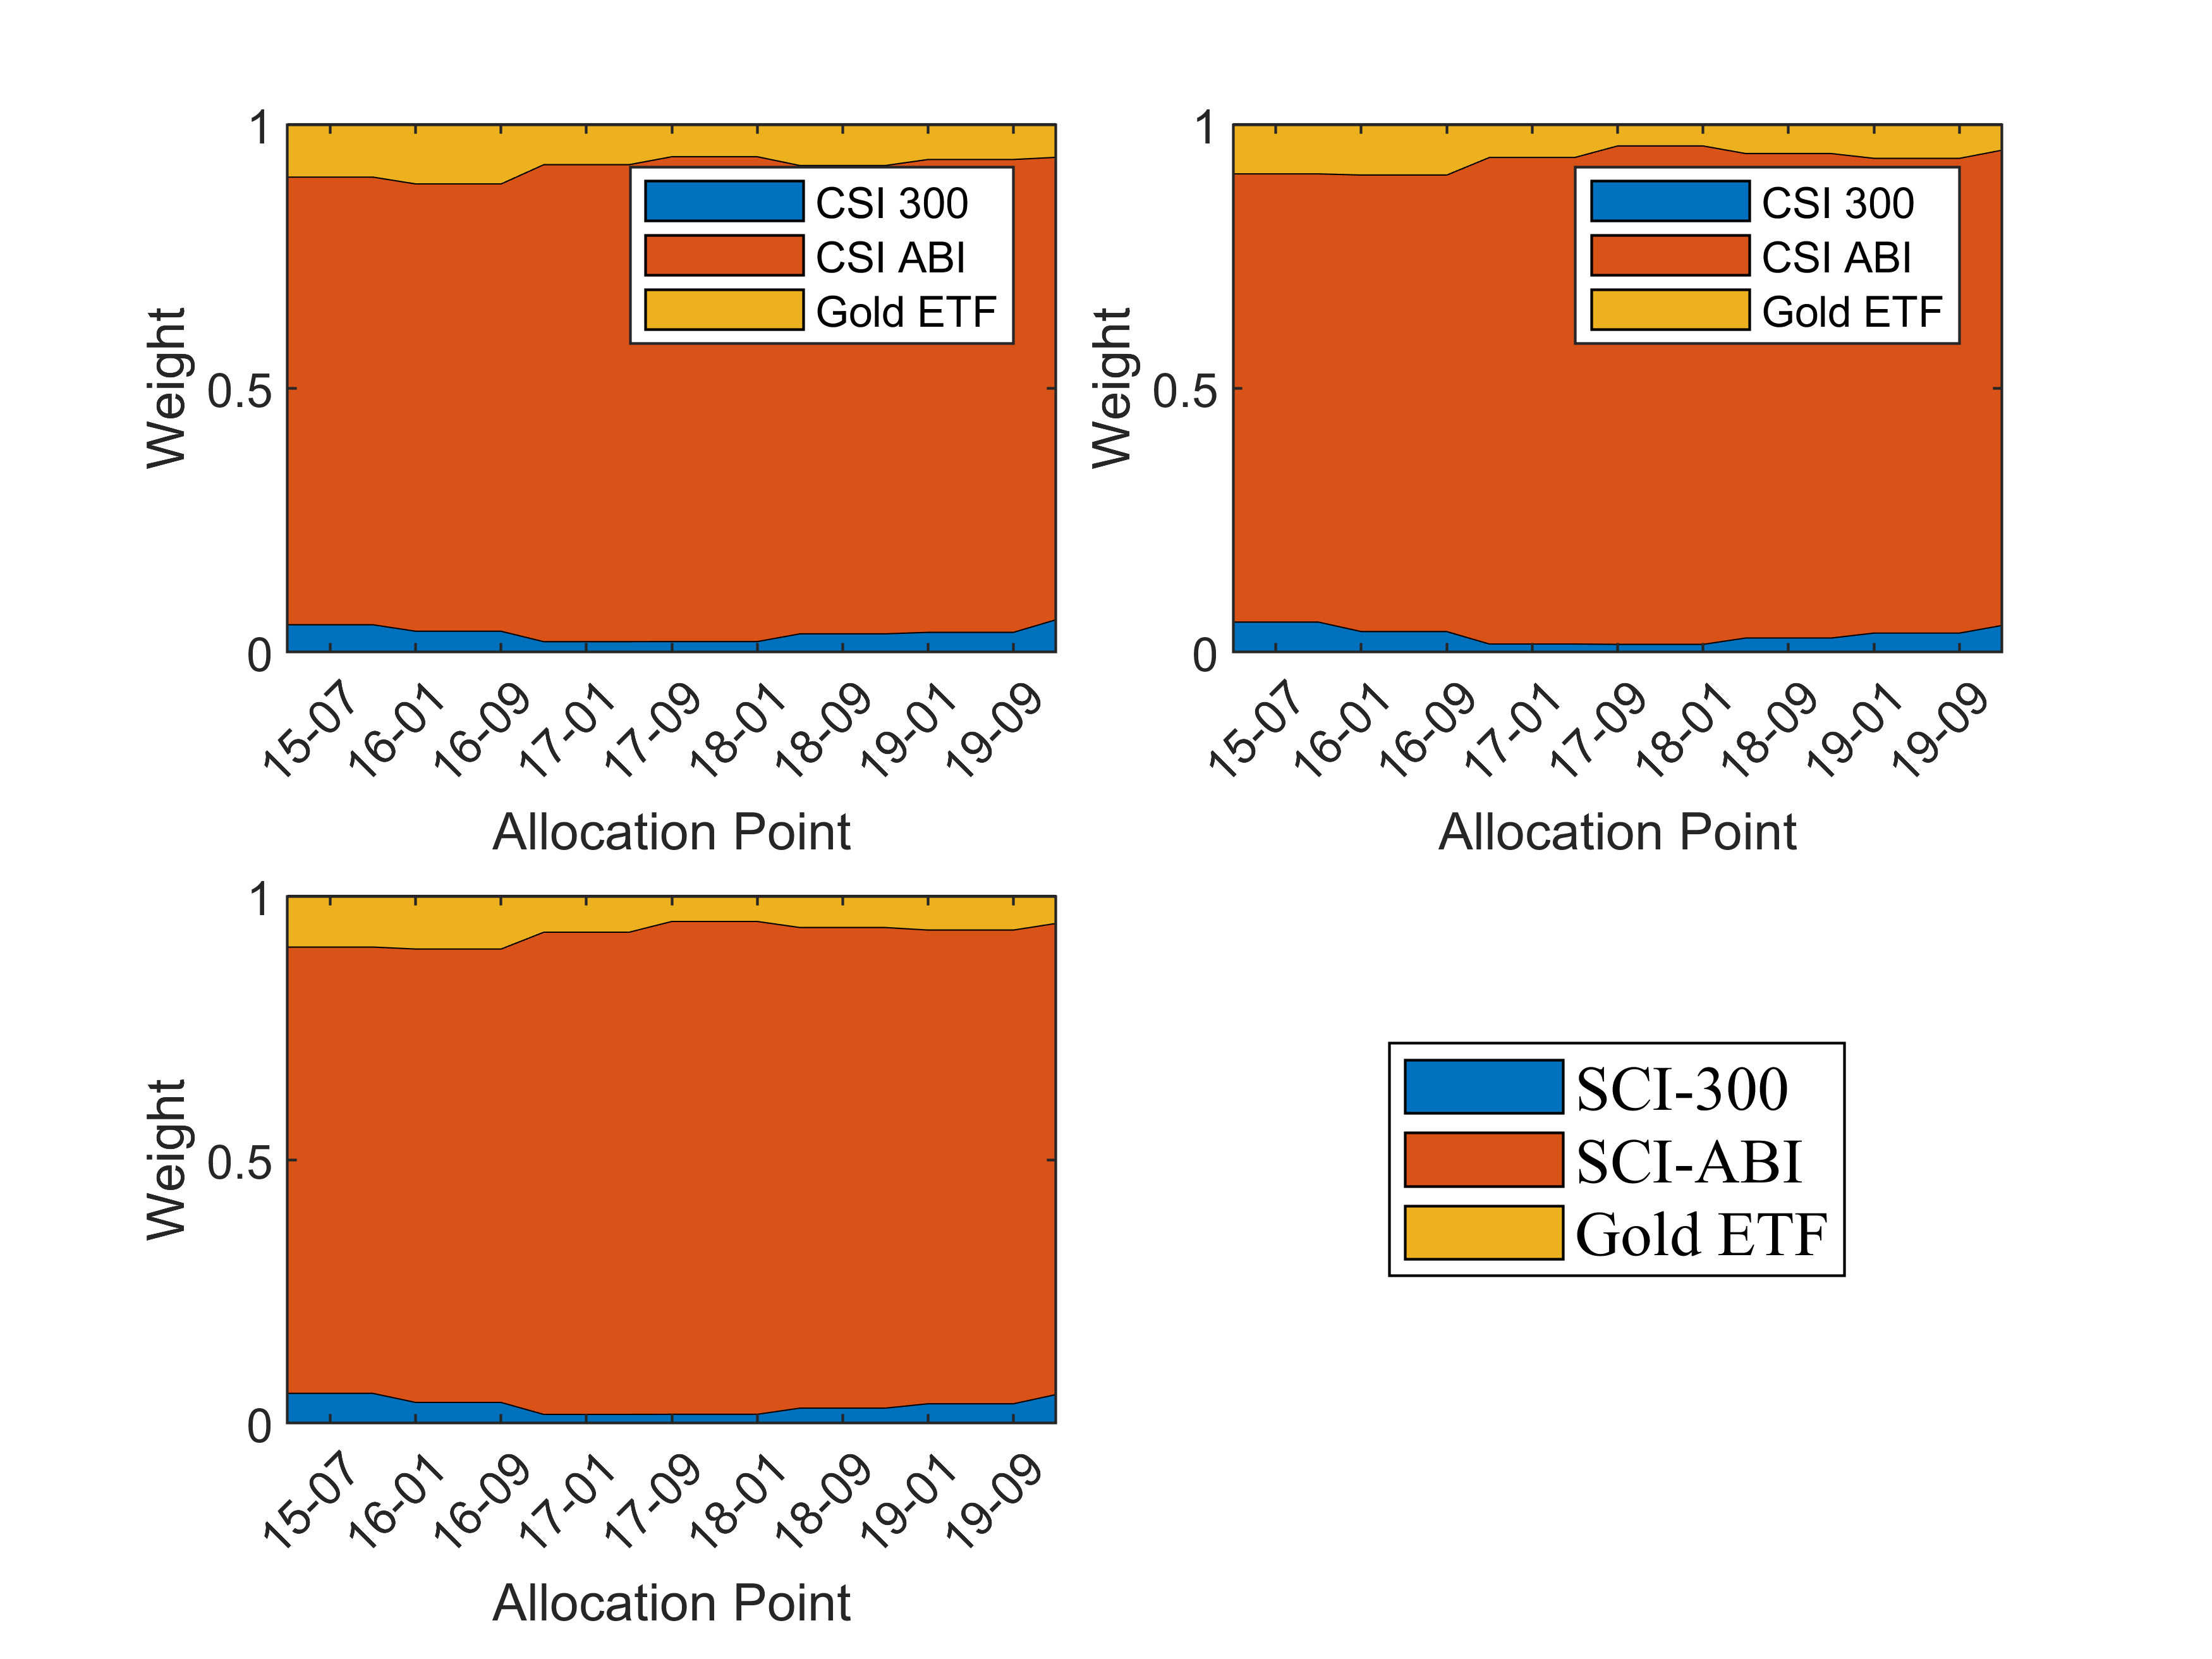
\includegraphics[scale=0.9]{Figure/FIG5-Allocation_Weight.png}
    \caption{The weight of assets based on Std Model(upper left), VaR Model (upper right), and ES Model (lower left)}
    \label{Fig5}
\end{figure}

\subsubsection{Analysis and Evaluation}
\paragraph{Allocation Models all outperform Individual Assets}\mbox{}\\
From the various evaluation indicators in \textbf{Table \ref{Tab3}}, we can find that the three allocation models have the following characteristics: (1) The annualized rate of return is higher than that of CSI 300 and CSI ABI, and lower than gold ETF; (2) The annualized volatility is much lower than that of CSI 300 and gold ETF, while it is slightly higher than that of CSI ABI. The maximum drawdown rate is lower than that of all individual assets; (3) Sharpe ratio is significant higher than that of a single asset.
This shows that through the asset allocation, financial risks have been dispersed adequately, and the overall performance of the asset portfolio is significantly better than that of a single asset.

\paragraph{Different models have their own characteristics}\mbox{}\\
Compared with the standard deviation models, the performance of the VaR model and the ES model is basically the same, both have higher annual returns, lower volatility and maximum drawdown than the standard deviation model. With respect to the Sharpe ratio, the standard deviation model is the lowest and the expected shortfall model is the highest. This is because the standard deviation indicator treats downside risk and upside risk equally. In other words, the standard deviation model overestimates the risk level of financial assets during the rising period, so that it could miss the investment opportunities when the "bull market" comes. 


\paragraph{Weight allocation with more debt and less shares}\mbox{}\\
According to the average weights of the three models allocated on various assets during the backtest period shown in \textbf{Table \ref{Tab4}}, it can be seen that the average allocation ratio of the VaR model is the lowest in the CSI 300 Index and the gold ETF, and the highest in the CSI ASI. The expected shortfall model is more sensitive to the changes of the upward and downward trend, so the allocation weight of stocks and gold ETF are slightly higher than VaR model. Finally, we also found that among three models, all of them have shown a significant feature of asset allocation ratio having more bonds than stocks, which is consistent with the fluctuation characteristics of assets.
